% ============================================================================
% EMCH 501: Engineering Analysis I - Assignment 3
% ============================================================================

\documentclass[12pt]{article}

% ============================================================================
% PACKAGE IMPORTS
% ============================================================================
\usepackage{amsmath}        % Advanced math symbols and equations
\usepackage{graphicx}       % Insert images/figures into your document
\usepackage{amssymb}        % Additional math symbols (like ℝ, ℕ, etc.)
\usepackage{tikz}           % Create diagrams and drawings directly in LaTeX
\usepackage[margin=1in]{geometry}  % Set page margins to 1 inch on all sides
\usepackage{setspace}       % Control line spacing (single, double, etc.)
\usepackage{xcolor}         % Use colors in your document
\usepackage{enumitem}       % Customize lists (bullets, numbers, etc.)
\usepackage{tcolorbox}      % Create colored boxes for hints, steps, etc.
\usepackage{fancyhdr}       % Customize headers and footers
\usepackage{lastpage}       % Reference the last page number (for "Page X of Y")

% Graphics and Colors
\usepackage{xcolor}
\usepackage{tcolorbox}
\usepackage{pgfplots}
\usepackage{listings}


% ============================================================================
% HEADER AND FOOTER SETUP
% ============================================================================
% This creates a header at the top of each page with page numbers and info
\pagestyle{fancy}              % Use the fancy page style
\setlength{\headheight}{14.5pt}  % Avoid LaTeX warning about header height
\fancyhf{}                     % Clear all header and footer fields

% Customize these three lines for your header:
\fancyhead[L]{Page \thepage\ of \pageref{LastPage}}  % Left: Page numbers
\fancyhead[C]{EMCH 501}     % Center: Your course code (CHANGE THIS!)
\fancyhead[R]{JC Vaught}       % Right: Your name (CHANGE THIS!)

\renewcommand{\headrulewidth}{0pt}  % Remove line under header (set to 2pt to add line)

% ============================================================================
% TIKZ LIBRARIES (for diagrams)
% ============================================================================
% Only needed if you're creating diagrams with TikZ
\usetikzlibrary{shapes.geometric, arrows.meta, positioning, decorations.pathmorphing, patterns}

% --- USC Brand Colors ---
\definecolor{USC_Garnet}{HTML}{73000A}
\definecolor{USC_Sandstorm}{HTML}{FFF2E3}
\definecolor{USC_Black90}{HTML}{565656}  % 90% black
\definecolor{USC_Black10}{HTML}{ECECEC}  % 10% black
\definecolor{USC_Honeycomb}{HTML}{65780B}


% ============================================================================
% CUSTOM COLORED BOXES
% ============================================================================
\newtcolorbox{stepbox}{
  colback=white,      % Light Sandstorm background
  colframe=USC_Garnet,        % Garnet border
  fonttitle=\bfseries,
  title=Step,
  sharp corners,
  colbacktitle=USC_Garnet,    % Garnet title bar
  coltitle=white,             % White title text
}

% CODE BOX - Neutral USC greys
\newtcolorbox{codebox}{
  colback=USC_Black10,        % Very light grey background
  colframe=USC_Black90,       % Dark grey border
  fonttitle=\bfseries,
  title=MATLAB Implementation,
  sharp corners,
  colbacktitle=USC_Black90,   % Dark grey title bar
  coltitle=white,             % White title text
}

% RESULTS BOX - Honeycomb accent
\newtcolorbox{resultsbox}{
  colback=white,      % Light Sandstorm background
  colframe=USC_Honeycomb,     % Honeycomb border
  fonttitle=\bfseries,
  title=Results,
  sharp corners,
  colbacktitle=USC_Honeycomb, % Honeycomb title bar
  coltitle=white,             % Black title text for contrast
}


% ============================================================================
% CUSTOM QUESTION COMMAND
% ============================================================================
% This creates a consistent format for each question with a double line separator

\newcommand{\question}[1]{%
  \clearpage                  % Start each question on a new page
  \vspace{0.5cm}             % Add vertical space
  {\noindent\normalsize \textbf{#1}}  % Bold question text
  \vspace{0.2cm}
  \hrule                     % First horizontal line
  \vspace{0.1cm}
  \hrule                     % Second horizontal line
  \vspace{0.3cm}
}

% Code listing style
\lstset{
    language=Matlab,
    basicstyle=\ttfamily\small,
    keywordstyle=\color{blue},
    commentstyle=\color{USC_Honeycomb},
    stringstyle=\color{USC_Garnet},
    breaklines=true,
    showstringspaces=false,
    backgroundcolor=\color{USC_Black10}
}
% ============================================================================
% DOCUMENT INFORMATION
% ============================================================================

\title{EMCH 501: Engineering Analysis I \\ Assignment 3}
\author{Instructor: Yi Wang, Department of Mechanical Engineering \\ University of South Carolina}
\date{Due: November 19, 2025}

% ============================================================================
% BEGIN DOCUMENT
% ============================================================================

\begin{document}

\maketitle
\setlength{\parindent}{0pt}

% ============================================================================
% LIST FORMATTING
% ============================================================================

\setlist[enumerate,1]{label=\arabic*.}
\setlist[enumerate,2]{label=\alph*.}

% ============================================================================
% TABLE OF CONTENTS
% ============================================================================

\begin{center}
\begin{tcolorbox}[colback=white, colframe=gray!50!black, colbacktitle=gray!20!white,
                  coltitle=black, sharp corners, boxrule=1pt,
                  title=\Large\bfseries Table of Contents]
\begin{tabular}{p{0.82\textwidth}r}
\textbf{Exercise 11.1: Problem 12 (6 pts)} \dotfill & \textbf{\pageref{quest:1}} \\
\textbf{Exercise 11.2: Problem 15 (6 pts)} \dotfill & \textbf{\pageref{quest:2}} \\
\textbf{Exercise 11.3: Problem 28 (4 pts)} \dotfill & \textbf{\pageref{quest:3}} \\
\textbf{Exercise 11.3: Problem 45 (10 pts)} \dotfill & \textbf{\pageref{quest:4}} \\
\textbf{Exercise 11.4: Problem 1 (15 pts)} \dotfill & \textbf{\pageref{quest:5}} \\
\textbf{Exercise 12.1: Problem 17 (3 pts)} \dotfill & \textbf{\pageref{quest:6}} \\
\textbf{Exercise 12.1: Problem 19 (3 pts)} \dotfill & \textbf{\pageref{quest:7}} \\
\textbf{Exercise 12.2: Problem 3 (4 pts)} \dotfill & \textbf{\pageref{quest:8}} \\
\textbf{Exercise 12.2: Problem 10 (4 pts)} \dotfill & \textbf{\pageref{quest:9}} \\
\textbf{Exercise 12.3: Problem 2 (10 pts)} \dotfill & \textbf{\pageref{quest:10}} \\
\textbf{Exercise 12.3: Problem 10 (15 pts)} \dotfill & \textbf{\pageref{quest:11}} \\
\textbf{Exercise 12.4: Problem 11 (8 pts)} \dotfill & \textbf{\pageref{quest:12}} \\
\textbf{Exercise 12.5: Problem 16 (12 pts)} \dotfill & \textbf{\pageref{quest:13}} \\
\end{tabular}
\vspace{0.2cm}
\end{tcolorbox}
\end{center}

\vspace{0.5cm}

% ============================================================================
% PROBLEM 1: Exercise 11.1 Problem 12
% ============================================================================

\question{Exercise 11.1: Problem 12 (6 pts)}\label{quest:1}

Show that the given set of functions is orthogonal on the indicated interval. Find the norm of each function in the set:

\begin{equation*}
\left\{1, \cos\frac{n\pi x}{p}, \sin\frac{m\pi x}{p}\right\} \quad \text{for each } m = 1,2,3,\ldots \text{ and } n = 1,2,3,\ldots 
\text{ on} [-p, p]
\end{equation*}
\textbf{NOTE:} Don't forget to show that $\cos\left(\frac{a\pi x}{p}\right)$ and $\cos\left(\frac{b\pi x}{p}\right)$ are orthogonal for $a \neq b$,
and that $\sin\left(\frac{a\pi x}{p}\right)$ and $\sin\left(\frac{b\pi x}{p}\right)$ are orthogonal for $a \neq b$.

\begin{stepbox}
For functions $f(x)$ and $g(x)$ on $[-p, p]$, the inner product is defined as:
\[ \langle f, g \rangle = \int_{-p}^{p} f(x)g(x) \, dx \]
The set is orthogonal if $\langle f, g \rangle = 0$ for any distinct pair of functions. The norm is $\|f\| = \sqrt{\langle f, f \rangle}$.
\end{stepbox}

\begin{stepbox}
Test the constant function $1$ against cosine
    \[ \int_{-p}^{p} 1 \cdot \cos\frac{n\pi x}{p} \, dx = \left[ \frac{p}{n\pi} \sin\frac{n\pi x}{p} \right]_{-p}^{p} = \frac{p}{n\pi} (\sin(n\pi) - \sin(-n\pi)) = 0 \]
\end{stepbox}

\begin{stepbox}  
Test the constant function $1$ against sine.\\
The function $\sin\frac{m\pi x}{p}$ is an \textbf{odd} function. \\
Integrating an odd function over a symmetric interval $[-p, p]$ yields 0.
    \[ \int_{-p}^{p} 1 \cdot \sin\frac{m\pi x}{p} \, dx = 0 \]
Thus, $1$ is orthogonal to all sine and cosine terms.
\end{stepbox}

\begin{stepbox}
Consider the product of any sine and cosine term:
\[ I = \int_{-p}^{p} \sin\frac{m\pi x}{p} \cos\frac{n\pi x}{p} \, dx \]
The integrand is the product of an odd function ($\sin$) and an even function ($\cos$), which results in an \textbf{odd} function.
\[ \text{Odd } \times \text{ Even } = \text{Odd} \]
Therefore, the integral over the symmetric interval $[-p, p]$ is zero.
\end{stepbox}

\begin{stepbox}
Using the identity $\cos A \cos B = \frac{1}{2}[\cos(A-B) + \cos(A+B)]$:
\[ \int_{-p}^{p} \cos\frac{n\pi x}{p} \cos\frac{k\pi x}{p} \, dx = \frac{1}{2} \int_{-p}^{p} \left[ \cos\frac{(n-k)\pi x}{p} + \cos\frac{(n+k)\pi x}{p} \right] dx \]
Since $n \neq k$, the arguments are non-zero integers times $\frac{\pi x}{p}$. The integral of cosine over integer periods (or symmetric bounds resolving to sine of integer $\pi$) is zero.
\end{stepbox}

\begin{stepbox}
Using the identity $\sin A \sin B = \frac{1}{2}[\cos(A-B) - \cos(A+B)]$:
\[ \int_{-p}^{p} \sin\frac{m\pi x}{p} \sin\frac{k\pi x}{p} \, dx = \frac{1}{2} \int_{-p}^{p} \left[ \cos\frac{(m-k)\pi x}{p} - \cos\frac{(m+k)\pi x}{p} \right] dx \]
Similar to step 3, since $m \neq k$, both cosine terms integrate to zero over $[-p, p]$.
\end{stepbox}

\begin{stepbox}
The square of the norm is $\|f\|^2 = \int_{-p}^p f^2(x) dx$.

\begin{enumerate}
    \item \textbf{Norm of 1:}
    \[ \|1\|^2 = \int_{-p}^{p} 1^2 \, dx = [x]_{-p}^{p} = 2p \implies \boxed{\|1\| = \sqrt{2p}} \]
    
    \item \textbf{Norm of Cosine ($n \neq 0$):}
    \[ \|\cos\|^2 = \int_{-p}^{p} \cos^2\frac{n\pi x}{p} \, dx = \int_{-p}^{p} \left(\frac{1 + \cos(2n\pi x/p)}{2}\right) dx \]
    The $\cos$ term integrates to 0.
    \[ = \int_{-p}^{p} \frac{1}{2} \, dx = p \implies \boxed{\|\cos\| = \sqrt{p}} \]
    
    \item \textbf{Norm of Sine ($m \neq 0$):}
    \[ \|\sin\|^2 = \int_{-p}^{p} \sin^2\frac{m\pi x}{p} \, dx = \int_{-p}^{p} \left(\frac{1 - \cos(2m\pi x/p)}{2}\right) dx = p \]
    \[ \implies \boxed{\|\sin\| = \sqrt{p}} \]
\end{enumerate}
\end{stepbox}

\begin{resultsbox}
\textbf{Summary of Norms:}
\begin{itemize}
    \item $\|1\| = \sqrt{2p}$
    \item $\|\cos\frac{n\pi x}{p}\| = \sqrt{p}$
    \item $\|\sin\frac{m\pi x}{p}\| = \sqrt{p}$
\end{itemize}
The set is orthogonal on $[-p, p]$.
\end{resultsbox}

\newpage

\begin{codebox}
\begin{lstlisting}
% Parameter Setup
p = 3;
x = linspace(-p, p, 1000);

% Define Functions
n = 2; m = 3;
f1 = cos(n*pi*x/p);
f2 = sin(m*pi*x/p);
prod = f1 .* f2;

% Calculate Inner Product (Numerical Integration)
inner_product = trapz(x, prod);

% Visualization
figure();
subplot(2,1,1);
plot(x, f1, 'b', 'LineWidth', 1.5, 'DisplayName', 'cos(2\pi x/p)'); hold on;
plot(x, f2, 'r', 'LineWidth', 1.5, 'DisplayName', 'sin(3\pi x/p)');
title('Individual Functions'); legend; grid on;

subplot(2,1,2);
% Split positive and negative parts for specific coloring
area(x, max(prod, 0), 'FaceColor', 'b', 'FaceAlpha', 0.5);
hold on;
area(x, min(prod, 0), 'FaceColor', 'r', 'FaceAlpha', 0.5);

yline(0, 'k-', 'LineWidth', 1);
title(['Product f1 * f2 (Area \approx ' num2str(inner_product) ')']);
subtitle('Positive (blue) and negative (red) areas cancel out');
xlabel('x'); grid on;
\end{lstlisting}
\end{codebox}

            \begin{resultsbox}
\centering
\includegraphics[width=1\linewidth]{problem_ortho.png}

\vspace{0.5em}
\small\textit{The shaded area represents the inner product integral. Due to the symmetry of the interval and the odd nature of the product function, the positive areas exactly cancel the negative areas, resulting in zero net area (orthogonality).}
\end{resultsbox}




% ============================================================================
% PROBLEM 2: Exercise 11.2 Problem 15
% ============================================================================

\question{Exercise 11.2: Problem 15 (6 pts)}\label{quest:2}

Find the Fourier series of $f$ on the given interval.

\begin{equation*}
f(x) = e^x, \quad -\pi < x < \pi
\end{equation*}


\begin{stepbox}
The general Fourier series for a function with period $2\pi$ is given by:
\[ f(x) \sim \frac{a_0}{2} + \sum_{n=1}^{\infty} (a_n \cos nx + b_n \sin nx) \]
First, we calculate the coefficient $a_0$:
\[ a_0 = \frac{1}{\pi} \int_{-\pi}^{\pi} e^x \, dx = \frac{1}{\pi} [e^x]_{-\pi}^{\pi} = \frac{e^\pi - e^{-\pi}}{\pi} \]
\end{stepbox}

\begin{stepbox}
Using the identity $\sinh x = \frac{e^x - e^{-x}}{2}$, we can simplify this to:
\[ a_0 = \frac{2 \sinh \pi}{\pi} \]
\end{stepbox}

\begin{stepbox}
Next, we calculate the cosine coefficients $a_n$. We use the standard integral formula $\int e^{ax} \cos(bx) dx = \frac{e^{ax}}{a^2+b^2}(a \cos bx + b \sin bx)$.
\[ a_n = \frac{1}{\pi} \int_{-\pi}^{\pi} e^x \cos(nx) \, dx \]
\[ a_n = \frac{1}{\pi} \left[ \frac{e^x}{1+n^2}(\cos(nx) + n \sin(nx)) \right]_{-\pi}^{\pi} \]
\end{stepbox}

\begin{stepbox}
Since $\sin(n\pi) = \sin(-n\pi) = 0$ and $\cos(n\pi) = \cos(-n\pi) = (-1)^n$:
\[ a_n = \frac{1}{\pi(1+n^2)} \left( e^\pi (-1)^n - e^{-\pi} (-1)^n \right) \]
\[ a_n = \frac{(-1)^n}{\pi(1+n^2)} (e^\pi - e^{-\pi}) = \frac{2 (-1)^n \sinh \pi}{\pi(1+n^2)} \]
\end{stepbox}

\begin{stepbox}
Finally, we calculate the sine coefficients $b_n$ using $\int e^{ax} \sin(bx) dx = \frac{e^{ax}}{a^2+b^2}(a \sin bx - b \cos bx)$.
\[ b_n = \frac{1}{\pi} \int_{-\pi}^{\pi} e^x \sin(nx) \, dx \]
\[ b_n = \frac{1}{\pi} \left[ \frac{e^x}{1+n^2}(\sin(nx) - n \cos(nx)) \right]_{-\pi}^{\pi} \]
\end{stepbox}

\begin{stepbox}
Substituting limits:
\[ b_n = \frac{1}{\pi(1+n^2)} \left( e^\pi(0 - n(-1)^n) - e^{-\pi}(0 - n(-1)^n) \right) \]
\[ b_n = \frac{-n(-1)^n}{\pi(1+n^2)} (e^\pi - e^{-\pi}) = \frac{2n (-1)^{n+1} \sinh \pi}{\pi(1+n^2)} \]
\end{stepbox}

\begin{resultsbox}
Substituting $a_0, a_n, b_n$ back into the series form gives the final Fourier Series:
\begin{equation*}
e^x \sim \frac{\sinh \pi}{\pi} + \frac{2\sinh \pi}{\pi} \sum_{n=1}^{\infty} \frac{(-1)^n}{1+n^2} (\cos nx - n \sin nx)
\end{equation*}
\end{resultsbox}

\begin{codebox}
\begin{lstlisting}
% 1. Define Domain and Function
x = linspace(-pi, pi, 1000);
f_exact = exp(x);

% 2. Define Coefficients
SinhPi = sinh(pi);
a0 = (2 * SinhPi) / pi;

% Function handles for coefficients an and bn
get_an = @(n) (2 * (-1)^n * SinhPi) / (pi * (1 + n^2));
get_bn = @(n) (2 * n * (-1)^(n+1) * SinhPi) / (pi * (1 + n^2));

% 3. Compute Partial Sums
terms_to_plot = [1, 3, 5, 20];
colors = {'b', 'g', 'm', 'r'}; % Colors for different sums

figure('Color', 'w');
plot(x, f_exact, 'k', 'LineWidth', 2.5, 'DisplayName', 'f(x) = e^x');
hold on;
grid on;

for i = 1:length(terms_to_plot)
    N = terms_to_plot(i);
    f_approx = (a0 / 2) * ones(size(x)); % Start with a0/2
    
    for n = 1:N
        an = get_an(n);
        bn = get_bn(n);
        f_approx = f_approx + an * cos(n*x) + bn * sin(n*x);
    end
    
    plot(x, f_approx, 'Color', colors{i}, 'LineWidth', 1.2, ...
         'DisplayName', sprintf('N = %d Terms', N));
end

% 4. Formatting the Plot
title('Fourier Series Convergence for f(x) = e^x');
xlabel('x'); ylabel('f(x)');
legend('Location', 'northwest');
xlim([-pi pi]);
\end{lstlisting}
\end{codebox}

\begin{resultsbox}
\centering
\includegraphics[width=1\linewidth]{problem_fourier.png}

\vspace{0.5em}
\small\textit{Varying Fourier expansions/approximations.}
\end{resultsbox}


% ============================================================================
% PROBLEM 3: Exercise 11.3 Problem 28
% ============================================================================

\question{Exercise 11.3: Problem 28 (4 pts)}\label{quest:3}

Find the half-range cosine and sine expansions for

\begin{equation*}
f(x) = \sin x, \quad 0 < x < \pi
\end{equation*}


\begin{stepbox}
Extend $f(x)$ as an \textbf{even} function on $-\pi < x < \pi$. The series is:
\[ f(x) = \frac{a_0}{2} + \sum_{n=1}^{\infty} a_n \cos(nx) \]
First, calculate $a_0$:
\[ a_0 = \frac{2}{L} \int_0^L f(x) dx = \frac{2}{\pi} \int_0^\pi \sin x \, dx = \frac{2}{\pi} [-\cos x]_0^\pi = \frac{2}{\pi}(1 - (-1)) = \frac{4}{\pi} \]
\end{stepbox}

\begin{stepbox}
Next, calculate $a_n$:
\[ a_n = \frac{2}{\pi} \int_0^\pi \sin x \cos nx \, dx \]
Using the identity $\sin A \cos B = \frac{1}{2}[\sin(A+B) + \sin(A-B)]$:
\[ a_n = \frac{1}{\pi} \int_0^\pi [\sin((1+n)x) + \sin((1-n)x)] \, dx \]
\end{stepbox}

\begin{stepbox}
\textbf{Case 1: $n=1$.} Since $\int_0^\pi \sin x \cos x \, dx = 0$ (orthogonality), $a_1 = 0$.

\textbf{Case 2: $n > 1$.}
\[ a_n = \frac{1}{\pi} \left[ \frac{-\cos(1+n)x}{1+n} - \frac{\cos(1-n)x}{1-n} \right]_0^\pi \]
\[ a_n = \frac{1}{\pi} \left( \left[ \frac{-\cos((1+n)\pi)}{1+n} - \frac{\cos((1-n)\pi)}{1-n} \right] - \left[ \frac{-1}{1+n} - \frac{-1}{1-n} \right] \right) \]
If $n$ is odd ($n=3,5,\dots$), terms cancel out to zero.
If $n$ is even ($n=2k$), $\cos((1+n)\pi) = -1$. The expression simplifies to:
\[ a_{2k} = \frac{-4}{\pi(4k^2-1)}, \quad k=1, 2, 3 \dots \]
\end{stepbox}

\begin{stepbox}
The series is:
\[ f(x) = \sum_{n=1}^{\infty} b_n \sin(nx) \]
Since $f(x) = \sin(x)$ is already a sine function matching the fundamental frequency of the interval $(0, \pi)$, this expansion is trivial by inspection.
\[ b_1 = 1, \quad b_n = 0 \text{ for } n > 1 \]
\end{stepbox}

\begin{resultsbox}
\textbf{Final Expansions:}

1. Half-Range Cosine Series (Even extension):
\[ f(x) = \frac{2}{\pi} - \frac{4}{\pi} \sum_{k=1}^{\infty} \frac{\cos(2kx)}{4k^2-1} \]

2. Half-Range Sine Series (Odd extension):
\[ f(x) = \sin x \]
\end{resultsbox}

\begin{codebox}
\begin{lstlisting}
% MATLAB Code to visualize the expansions
x = linspace(-pi, pi, 1000); % Plot from -pi to pi to show symmetry
f_target = abs(sin(x)); % The even extension of sin(x) on (0,pi)

% 1. Sine Expansion (Trivial)
f_sine = sin(x); % The odd extension

% 2. Cosine Expansion (Partial Sum)
N = 10; % Number of terms
a0 = 4/pi;
f_cosine = zeros(size(x)) + a0/2;

for k = 1:N
    n = 2*k; % Even terms only
    an = -4 / (pi * (4*k^2 - 1));
    f_cosine = f_cosine + an * cos(n*x);
end

% Plotting
figure('Color', 'w');
subplot(2,1,1);
plot(x, f_sine, 'r-', 'LineWidth', 2); hold on;
x_orig = linspace(0, pi, 500);
plot(x_orig, sin(x_orig), 'k--', 'LineWidth', 2);
title('Half-Range Sine Expansion (Odd Extension)');
legend('Expansion', 'Original f(x)'); grid on;

subplot(2,1,2);
plot(x, f_cosine, 'b-', 'LineWidth', 2); hold on;
plot(x, f_target, 'k:', 'LineWidth', 1.5);
title(['Half-Range Cosine Expansion (Even Extension, N=', num2str(N), ')']);
legend('Approximation', 'Target |sin(x)|'); grid on;
\end{lstlisting}
\end{codebox}

\begin{resultsbox}
\centering
\includegraphics[width=1\linewidth]{problem_expansion.png}

\vspace{0.5em}
\small\textit{The Sine expansion (Red) extends the function oddly into $x<0$. \\
The Cosine expansion (Blue) extends the function evenly (absolute value shape).}
\end{resultsbox}


% ============================================================================
% PROBLEM 4: Exercise 11.3 Problem 45
% ============================================================================

\question{Exercise 11.3: Problem 45 (10 pts)}\label{quest:4}

An undamped spring/mass system with mass $m = \frac{1}{4}$ slug and spring constant $k = 12$ lb/ft is driven by a 2-periodic external force $f(t)$. Find a particular solution $x_p(t)$ to the differential equation of motion:

\begin{equation*}
m\frac{d^2x}{dt^2} + kx = f(t)
\end{equation*}

where the driving force is:
\begin{equation*}
f(t) = 2\pi t - t^2, \quad 0 < t < 2\pi; \quad f(t + 2\pi) = f(t)
\end{equation*}

Assume that when $f(t)$ is extended to the negative $t$-axis in a periodic manner, the resulting function is \textbf{even}.

\begin{figure}[h]
    \centering
    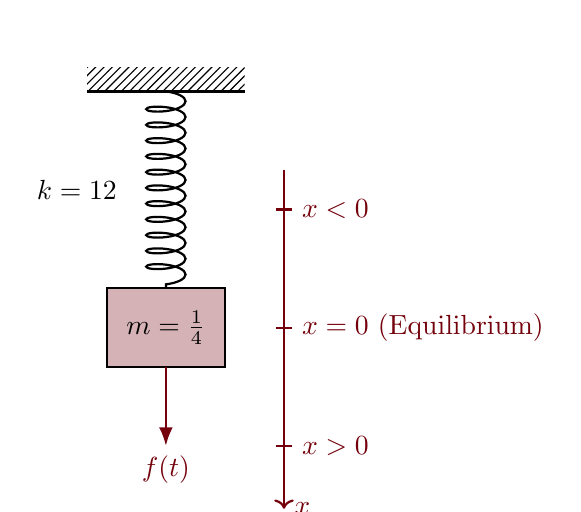
\begin{tikzpicture}[scale=1]
        
        % --- 1. Physical System Diagram (Left Side) ---
        
        % Support/Ceiling
        \fill[pattern=north east lines] (-1, 0) rectangle (1, 0.3);
        \draw[thick] (-1, 0) -- (1, 0);
        
        % Spring (Resting/Equilibrium position roughly)
        \draw[decoration={aspect=0.3, segment length=2mm, amplitude=2.5mm, coil}, decorate, thick] (0,0) -- (0,-2.5);
        
        % Mass
        \draw[fill= USC_Garnet!30, thick] (-0.75, -2.5) rectangle (0.75, -3.5);
        \node at (0, -3) {$m=\frac{1}{4}$};
        
        % Coordinate System (x-axis pointing down)
        \draw[->, thick, USC_Garnet] (1.5, -1) -- (1.5, -5.3) node[right] {$x$};
        \draw[thick, USC_Garnet] (1.4, -3.0) -- (1.6, -3.0) node[right] {$x=0$ (Equilibrium)};
        \draw[thick, USC_Garnet] (1.4, -1.5) -- (1.6, -1.5) node[right] {$x < 0$};
        \draw[thick, USC_Garnet] (1.4, -4.5) -- (1.6, -4.5) node[right] {$x > 0$};

        % Force Vector
        \draw[-Latex, USC_Garnet, thick] (0, -3.5) -- (0, -4.5) node[below] {$f(t)$};

        % Labels
        \node[anchor=east] at (-0.5, -1.25) {$k=12$};


    \end{tikzpicture}
    \caption{The undamped spring-mass system. }
\end{figure}


\begin{stepbox}
Substitute the physical parameters into the equation of motion:
\[ \frac{1}{4} x'' + 12x = f(t) \]
Multiplying the entire equation by 4 to normalize the derivative term:
\[ x'' + 48x = 4f(t) \]
The natural frequency of the system is $\omega_0 = \sqrt{48} = 4\sqrt{3} \approx 6.93$ rad/s.
\end{stepbox}

\begin{stepbox}
Determine the Fourier Series representation of the forcing function $F(t) = 4f(t)$.
Since $f(t)$ is \textbf{even} with period $2\pi$, we use a Fourier Cosine Series:
\[ f(t) = \frac{a_0}{2} + \sum_{n=1}^{\infty} a_n \cos(nt) \]

Calculating $a_0$:
\[ a_0 = \frac{2}{\pi} \int_0^{\pi} (2\pi t - t^2) dt \quad \text{OR} \quad a_0 = \frac{1}{\pi} \int_0^{2\pi} (2\pi t - t^2) dt \]
\[ a_0 = \frac{1}{\pi} \left[ \pi t^2 - \frac{t^3}{3} \right]_0^{2\pi} = \frac{1}{\pi} \left( 4\pi^3 - \frac{8\pi^3}{3} \right) = \frac{4\pi^2}{3} \]
\end{stepbox}

\begin{stepbox}
Calculating $a_n$:
\[ a_n = \frac{1}{\pi} \int_0^{2\pi} (2\pi t - t^2) \cos(nt) dt \]
Using integration by parts twice:
\[ a_n = -\frac{4}{n^2} \]
Thus, the driving force term $4f(t)$ is:
\[ 4f(t) = 4\left( \frac{2\pi^2}{3} - \sum_{n=1}^{\infty} \frac{4}{n^2} \cos(nt) \right) = \frac{8\pi^2}{3} - \sum_{n=1}^{\infty} \frac{16}{n^2} \cos(nt) \]
\end{stepbox}

\begin{stepbox}
We assume a particular solution of the form:
\[ x_p(t) = \frac{A_0}{2} + \sum_{n=1}^{\infty} A_n \cos(nt) \]
Substituting $x_p$ into the ODE $x'' + 48x = 4f(t)$:
\[ \sum_{n=1}^{\infty} -n^2 A_n \cos(nt) + 48 \left( \frac{A_0}{2} + \sum_{n=1}^{\infty} A_n \cos(nt) \right) = \frac{8\pi^2}{3} - \sum_{n=1}^{\infty} \frac{16}{n^2} \cos(nt) \]
\end{stepbox}

\begin{stepbox}
Matching coefficients:
\begin{enumerate}
    \item \textbf{Constant Term:} $24 A_0 = \frac{8\pi^2}{3} \implies A_0 = \frac{\pi^2}{9}$.
    \item \textbf{Cosine Terms:} $(48 - n^2)A_n = -\frac{16}{n^2} \implies A_n = \frac{-16}{n^2(48 - n^2)}$.
\end{enumerate}
\end{stepbox}

\begin{resultsbox}
The steady-state particular solution is:
\[ x_p(t) = \frac{\pi^2}{18} + 16\sum_{n=1}^{\infty} \frac{\cos(nt)}{n^2(n^2 - 48)} \]
\end{resultsbox}

\begin{codebox}
\begin{lstlisting}
L = pi;
t = linspace(0, 4*pi, 1000); % 2 periods
N_terms = 20;
% 1. Construct Forcing Function f(t) via Fourier Series
f_t = (2*pi^2)/3; % a0/2 term
for n = 1:N_terms
    an = -4 / n^2;
    f_t = f_t + an * cos(n*t);
end
% 2. Construct Response x(t)
x_t = (pi^2)/18; % A0/2 term
for n = 1:N_terms
    An = -16 / (n^2 * (48 - n^2));
    x_t = x_t + An * cos(n*t);
end
% Visualization
figure;
subplot(2,1,1);
plot(t, f_t, 'r', 'LineWidth', 1.5);
title('Forcing Function f(t) (Extended Even)');
ylabel('Force (lb)'); grid on; xlim([0 4*pi]);

subplot(2,1,2);
plot(t, x_t, 'b', 'LineWidth', 1.5);
title('System Response x_p(t)');
xlabel('Time (s)'); ylabel('Displacement (ft)');
grid on; xlim([0 4*pi]);
\end{lstlisting}
\end{codebox}

\begin{resultsbox}
\centering
\includegraphics[width=1\linewidth]{problem_spring.png}

\vspace{0.5em}
\small\textit{Generated plots showing the periodic parabolic forcing function and the resulting steady-state displacement.}
\end{resultsbox}


% ============================================================================
% PROBLEM 5: Exercise 11.4 Problem 1
% ============================================================================

\question{Exercise 11.4: Problem 1 (15 pts)}\label{quest:5}

Find the eigenfunctions and the equation that defines the eigenvalues for the given boundary-value problem.
Use a CAS to approximate the first four eigenvalues $\lambda_1, \lambda_2, \lambda_3,$ and $\lambda_4$.
Give the eigenfunctions corresponding to these approximations.

\begin{equation*}
y'' + \lambda y = 0
\end{equation*}

with boundary conditions:
\begin{equation*}
y'(0) = 0, \quad y'(1) + y(1) = 0
\end{equation*}


% ----------------------------------------------------------------------------
% SOLUTION STEPS
% ----------------------------------------------------------------------------

\begin{stepbox}
Let $\lambda = \alpha^2$ where $\alpha > 0$. The general solution to the ODE is:
\[ y(x) = c_1 \cos(\alpha x) + c_2 \sin(\alpha x) \]
Differentiation gives:
\[ y'(x) = -c_1 \alpha \sin(\alpha x) + c_2 \alpha \cos(\alpha x) \]
\end{stepbox}

\begin{stepbox}
Apply the first boundary condition $y'(0) = 0$:
\[ y'(0) = -c_1 \alpha (0) + c_2 \alpha (1) = 0 \implies c_2 = 0 \]
Thus, the eigenfunction simplifies to:
\[ y(x) = c_1 \cos(\alpha x) \]
\end{stepbox}

\begin{stepbox}
Apply the second boundary condition $y'(1) + y(1) = 0$:
\[ y'(1) = -c_1 \alpha \sin(\alpha) \]
\[ y(1) = c_1 \cos(\alpha) \]
Substituting these into the boundary condition:
\[ -c_1 \alpha \sin(\alpha) + c_1 \cos(\alpha) = 0 \]
\end{stepbox}

\begin{stepbox}
Assuming $c_1 \neq 0$ (for non-trivial solutions) and dividing by $\sin(\alpha)$ (assuming $\sin\alpha \neq 0$), we get the defining equation for the eigenvalues:
\[ \cos(\alpha) = \alpha \sin(\alpha) \quad \implies \quad \cot(\alpha) = \alpha \]
The eigenvalues are given by $\lambda_n = \alpha_n^2$, where $\alpha_n$ are the positive roots of $\cot \alpha = \alpha$.
\end{stepbox}


% ----------------------------------------------------------------------------
% CODE SECTION
% ----------------------------------------------------------------------------

\begin{codebox}
\begin{lstlisting}
fun = @(alpha) cot(alpha) - alpha;

% Initial guesses for the roots (near n*pi)
guesses = [0.5, 3.5, 6.5, 9.5];
alphas = zeros(1, 4);

% Solve for the first 4 roots
fprintf('n \t alpha_n \t lambda_n\n');
fprintf('-------------------------\n');
for i = 1:4
    alphas(i) = fzero(fun, guesses(i));
    lambdas(i) = alphas(i)^2;
    fprintf('%d \t %.4f \t %.4f\n', i, alphas(i), lambdas(i));
end

% Visualization Code
x = linspace(0, 1, 100);
figure; hold on;
labels = {};
for i = 1:4
    y = cos(alphas(i) * x);
    % Normalize for better plotting
    y = y / max(abs(y)); 
    plot(x, y, 'LineWidth', 1.5);
    labels{i} = sprintf('n=%d', i);
end
legend(labels);
title('First 4 Eigenfunctions y_n(x) = cos(\alpha_n x)');
grid on;
\end{lstlisting}
\end{codebox}

% ----------------------------------------------------------------------------
% RESULTS SECTION
% ----------------------------------------------------------------------------

\begin{resultsbox}
\textbf{Eigenvalues:}
Solving $\cot(\alpha) = \alpha$ numerically yields the roots $\alpha_n$. The eigenvalues are $\lambda_n = \alpha_n^2$.

\begin{center}
\begin{tabular}{c | c | c} 
 $n$ & Root ($\alpha_n$) & Eigenvalue ($\lambda_n$) \\
 \hline
 1 & 0.8603 & \textbf{0.7402} \\ 
 2 & 3.4256 & \textbf{11.7349} \\
 3 & 6.4373 & \textbf{41.4388} \\
 4 & 9.4248 & \textbf{88.8264} \\
\end{tabular}
\end{center}
\end{resultsbox}

\begin{resultsbox}
\textbf{Eigenfunctions:}
The corresponding eigenfunctions are:
\begin{center}
\begin{tabular}{c | c} 
 $n$ & Eigenfunction ($\cos(\alpha_n x)$)   \\
 \hline
 1 & $y_n(x) = \cos(0.8063 x)$ \\ 
 2 & $y_n(x) = \cos(3.4256 x)$ \\
 3 & $y_n(x) = \cos(6.4373 x)$ \\
 4 & $y_n(x) = \cos(9.4248 x)$ \\
\end{tabular}
\end{center}

\end{resultsbox}

\begin{resultsbox}
\centering
\includegraphics[width=1\linewidth]{problem_eigen.png}

\vspace{0.5em}
\small\textit{The plot shows the analytical steady-state solution}
\end{resultsbox}



% ============================================================================
% PROBLEM 6: Exercise 12.1 Problem 17
% ============================================================================

\question{Exercise 12.1: Problem 17 (3 pts)}\label{quest:6}

Classify the given partial differential equation as hyperbolic, parabolic, or elliptic:

\begin{equation*}
\frac{\partial^2 u}{\partial x^2} + \frac{\partial^2 u}{\partial x \partial y} + \frac{\partial^2 u}{\partial y^2} = 0
\end{equation*}

% --- Step 1: Identify Coefficients ---
\begin{stepbox}
The general form of a second-order linear partial differential equation in two variables $x$ and $y$ is given by:
\[ A \frac{\partial^2 u}{\partial x^2} + B \frac{\partial^2 u}{\partial x \partial y} + C \frac{\partial^2 u}{\partial y^2} + D \frac{\partial u}{\partial x} + E \frac{\partial u}{\partial y} + F u = G \]
Comparing this to the given equation:
\[ 1 \cdot u_{xx} + 1 \cdot u_{xy} + 1 \cdot u_{yy} = 0 \]
We identify the coefficients:
\begin{itemize}
    \item $A = 1$
    \item $B = 1$
    \item $C = 1$
\end{itemize}
\end{stepbox}

% --- Step 2: Compute Discriminant ---
\begin{stepbox}
The classification is determined by the sign of the discriminant $\Delta = B^2 - 4AC$.
\begin{itemize}
    \item If $\Delta > 0$, the equation is \textbf{Hyperbolic}.
    \item If $\Delta = 0$, the equation is \textbf{Parabolic}.
    \item If $\Delta < 0$, the equation is \textbf{Elliptic}.
\end{itemize}

Substituting our coefficients:
\[ \Delta = (1)^2 - 4(1)(1) \]
\[ \Delta = 1 - 4 \]
\[ \Delta = -3 \]
\end{stepbox}

% --- Final Result ---
\begin{resultsbox}
Since the discriminant $\Delta = -3 < 0$, the partial differential equation is classified:
\[ \textbf{Elliptic} \]
\end{resultsbox}

% ============================================================================
% PROBLEM 7: Exercise 12.1 Problem 19
% ============================================================================

\question{Exercise 12.1: Problem 19 (3 pts)}\label{quest:7}

Classify the given partial differential equation as hyperbolic, parabolic, or elliptic:

\begin{equation*}
\frac{\partial^2 u}{\partial x^2} + 6\frac{\partial^2 u}{\partial x \partial y} + 9\frac{\partial^2 u}{\partial y^2} = 0
\end{equation*}

\
\begin{stepbox}
The general form of a second-order linear partial differential equation in two variables is:
\[ A \frac{\partial^2 u}{\partial x^2} + B \frac{\partial^2 u}{\partial x \partial y} + C \frac{\partial^2 u}{\partial y^2} + D \frac{\partial u}{\partial x} + E \frac{\partial u}{\partial y} + F u = G \]
We identify the coefficients of the second-order terms from the given equation:
\[ A = 1, \quad B = 6, \quad C = 9 \]
\end{stepbox}

\begin{stepbox}
The classification of the PDE depends on the sign of the discriminant $\Delta$, defined as:
\[ \Delta = B^2 - 4AC \]
We substitute the identified coefficients into this formula:
\[ \Delta = (6)^2 - 4(1)(9) \]
\[ \Delta = 36 - 36 \]
\[ \Delta = 0 \]
\end{stepbox}

\begin{stepbox}
We apply the standard classification rules:
\begin{itemize}
    \item If $\Delta > 0$, the equation is \textbf{Hyperbolic}.
    \item If $\Delta = 0$, the equation is \textbf{Parabolic}.
    \item If $\Delta < 0$, the equation is \textbf{Elliptic}.
\end{itemize}
\end{stepbox}

\begin{resultsbox}
Since the discriminant $\Delta = 0$, the given partial differential equation is classified as:
\[ \textbf{Parabolic} \]
\end{resultsbox}


% ============================================================================
% PROBLEM 8: Exercise 12.2 Problem 3
% ============================================================================

\question{Exercise 12.2: Problem 3 (4 pts)}\label{quest:8}

A rod of length $L$ coincides with the interval $[0, L]$ on the $x$-axis. The left end is held at temperature 100, and there is heat transfer from the right end into the surrounding medium at temperature zero. The initial temperature is $f(x)$ throughout. Set up the boundary-value problem for the temperature $u(x,t)$.
\begin{figure}[htbp]
    \centering
    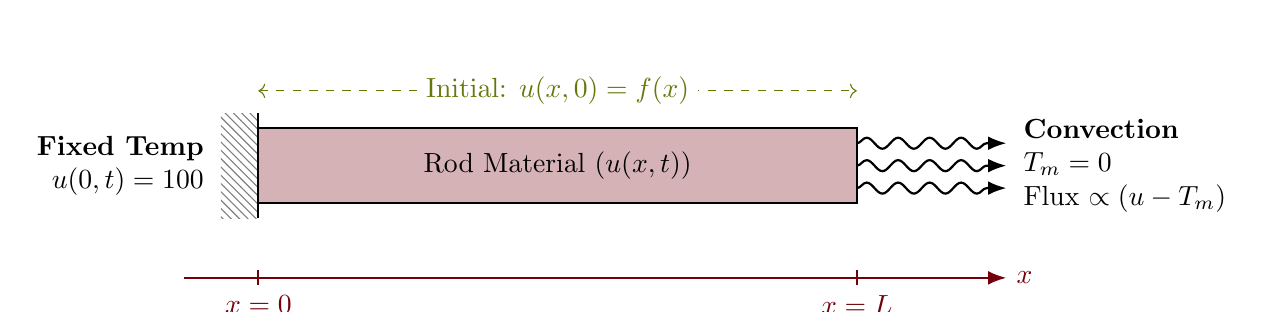
\begin{tikzpicture}[scale=0.95]
        % Parameters
        \def\RodLen{8}
        \def\RodH{1}
        
        % 1. Draw the Axis
        \draw[-Latex, thick, USC_Garnet] (-1, -1) -- (\RodLen + 2, -1) node[right] {$x$};
        
        % Ticks and labels
        \draw[thick, USC_Garnet] (0, -0.9) -- (0, -1.1) node[below] {$x=0$};
        \draw[thick, USC_Garnet] (\RodLen, -0.9) -- (\RodLen, -1.1) node[below] {$x=L$};
        
        % 2. Draw the Rod
        \draw[fill=USC_Garnet!30, thick] (0,0) rectangle (\RodLen, \RodH);
        \node at (\RodLen/2, \RodH/2) {Rod Material ($u(x,t)$)};
        
        % 3. Left Boundary Condition (Fixed Temp)
        \fill[pattern=north west lines, pattern color=gray] (-0.5, -0.2) rectangle (0, \RodH + 0.2);
        \draw[thick] (0, -0.2) -- (0, \RodH + 0.2);
        
        % Label for Left BC
        \node[anchor=east, align=right] at (-0.6, \RodH/2) {
            \textbf{Fixed Temp}\\
            $u(0,t) = 100$
        };
        
        % 4. Right Boundary Condition (Convection)
        \foreach \y in {0.2, 0.5, 0.8} {
            \draw[-Latex, thick, decorate, decoration={snake, amplitude=0.7mm, segment length=4mm, post length=2mm}] 
            (\RodLen, \y) -- (\RodLen + 2.0, \y);
        }
        
        % Label for Right BC
        \node[anchor=west, align=left] at (\RodLen + 2.1, \RodH/2) {
            \textbf{Convection}\\
            $T_m = 0$\\
            Flux $\propto (u - T_m)$
        };
        
        % 5. Initial Condition Label
        \draw[<->, dashed, USC_Honeycomb] (0, \RodH + 0.5) -- (\RodLen, \RodH + 0.5) node[midway, fill=white] {Initial: $u(x,0) = f(x)$};

    \end{tikzpicture}
    \caption{Schematic of the 1D heat equation problem with mixed boundary conditions.}
\end{figure}


\begin{stepbox}
For heat conduction in a one-dimensional rod without internal heat generation, the temperature $u(x,t)$ satisfies the standard heat equation:
\[ k \frac{\partial^2 u}{\partial x^2} = \frac{\partial u}{\partial t}, \quad 0 < x < L, \quad t > 0 \]
where $k > 0$ is the thermal diffusivity.
\end{stepbox}

\begin{stepbox}
Since the left end is held at a constant temperature of 100, this is a Dirichlet boundary condition:
\[ u(0, t) = 100, \quad t > 0 \]
\end{stepbox}

\begin{stepbox}
Since there is heat transfer into the surrounding medium at temperature zero at the right end, this describes convection, governed by Newton's Law of Cooling.
The heat flux is proportional to the temperature difference between the rod and the medium.
\begin{itemize}
    \item Fourier's Law (Heat Flux inside rod): $q = -K_{thermal} \frac{\partial u}{\partial x}$
    \item Newton's Law (Heat Flux at surface): $q = H (u(L,t) - T_m)$
\end{itemize}
\end{stepbox}

\begin{stepbox}
Equating fluxes at the boundary $x=L$:
\[ -K_{thermal} \frac{\partial u}{\partial x}\bigg|_{x=L} = H [u(L,t) - 0] \]
Rearranging terms and letting $h = H/K_{thermal}$ be a positive constant:
\[ \frac{\partial u}{\partial x}\bigg|_{x=L} + h u(L,t) = 0, \quad t > 0 \]
\end{stepbox}

\begin{stepbox}
Finally, the initial temperature distribution is given as a function $f(x)$.
\[ u(x, 0) = f(x), \quad 0 < x < L \]
\end{stepbox}

\begin{resultsbox}
The complete Boundary-Value Problem (BVP) is:

\textbf{PDE:}
\[ \frac{\partial^2 u}{\partial x^2} = \frac{1}{k} \frac{\partial u}{\partial t}, \quad 0 < x < L, \; t > 0 \]

\textbf{Boundary Conditions:}
\[ u(0, t) = 100 \]
\[ \frac{\partial u}{\partial x}(L, t) = -h u(L, t) \quad (\text{where } h > 0) \]

\textbf{Initial Condition:}
\[ u(x, 0) = f(x) \]
\end{resultsbox}

\newpage

\begin{codebox}

\begin{lstlisting}
function heat_eqn_bvp
    m = 0; % Symmetry parameter (0 for slab/rod)
    x = linspace(0, 1, 50);
    t = linspace(0, 0.5, 20);

    % Solve PDE
    sol = pdepe(m, @pdefun, @icfun, @bcfun, x, t);
    u = sol(:,:,1);

    % Plot
    figure;
    surf(x, t, u);
    title('Numerical Solution of the BVP');
    xlabel('Position x'); ylabel('Time t'); zlabel('Temp u');
    view([135 35]); colormap('jet');
end

% 1. PDE: ut = k*uxx
function [c,f,s] = pdefun(x,t,u,dudx)
    k = 1; % Diffusivity
    c = 1;
    f = k * dudx; % Flux term
    s = 0;        % Source term
end

% 2. Initial Condition: u(x,0) = f(x)
function u0 = icfun(x)
    u0 = 0; % Arbitrary initial temp f(x)
end

% 3. Boundary Conditions
function [pl,ql,pr,qr] = bcfun(xl,ul,xr,ur,t)
    % Left BC: u(0,t) = 100
    pl = ul - 100; 
    ql = 0; 
    
    % Right BC: ux(L,t) + h*u(L,t) = 0 
    % Flux f = k*ux. So ux = f/k.
    k = 1; h = 1;
    pr = k*h * ur; % Convection term
    qr = 1;        % Flux term coeff
end
\end{lstlisting}
\end{codebox}

\begin{resultsbox}
\centering
\includegraphics[width=1\linewidth]{problem_heat_bar.png}

\vspace{0.5em}
\small\textit{The plot shows the analytical steady-state solution}
\end{resultsbox}
% ============================================================================
% PROBLEM 9: Exercise 12.2 Problem 10
% ============================================================================

\question{Exercise 12.2: Problem 10 (4 pts)}\label{quest:9}

A string of length $L$ coincides with the interval $[0, L]$ on the $x$-axis. The ends are secured to the $x$-axis, and the string is initially at rest on that axis. An external vertical force proportional to the horizontal distance from the left end acts on the string for $t > 0$. Set up the boundary-value problem for displacement $u(x,t)$.

\begin{figure}[htbp]
\centering
\begin{tikzpicture}[scale=1.5, >=Stealth]
    % Axis
    \draw[->] (-0.5,0) -- (5.5,0) node[right] {$x$};
    \draw[->] (0,-0.5) -- (0,2.5) node[above] {$u(x,t)$};
    
    % String Constraints
    \draw[thick, color=USC_Garnet] (0,0) -- (5,0);
    \fill[USC_Garnet] (0,0) circle (2pt) node[below left] {$x=0$};
    \fill[USC_Garnet] (5,0) circle (2pt) node[below] {$x=L$};
    
    % Force Vectors (Proportional to x)
    \foreach \x in {0.5, 1.0, 1.5, 2.0, 2.5, 3.0, 3.5, 4.0, 4.5} {
        \draw[->, color=USC_Honeycomb, thick] (\x, 0.1) -- (\x, \x*0.4 + 0.1);
    }
    \node[color=USC_Honeycomb, anchor=west] at (5, 2) {Force $F(x) \propto x$};
\end{tikzpicture}
\caption{Diagram of the string initially at rest with an external force increasing linearly along the length of the string.}
\end{figure}


\begin{stepbox}
The standard one-dimensional wave equation describes the displacement $u(x,t)$ of a vibrating string. When an external force is applied, the equation becomes:
\[ a^2 \frac{\partial^2 u}{\partial x^2} + F_{\text{ext}} = \frac{\partial^2 u}{\partial t^2} \]
where:
\begin{itemize}
    \item $F_{\text{ext}}$ is the external force per unit mass.
    \item $a$ is the wave speed, related to tension $T$ and linear density $\rho$ by $a = \sqrt{T/\rho}$.
\end{itemize}
\end{stepbox}

\begin{stepbox}
Let $A$ be the constant of proportionality (where $A > 0$ implies an upward force).
\[ F_{\text{ext}}(x) = Ax \]
The constant $A$ represents the rate of change of force per unit mass along the string. Thus, the Partial Differential Equation (PDE) is:
\[ a^2 \frac{\partial^2 u}{\partial x^2} + Ax = \frac{\partial^2 u}{\partial t^2}, \quad 0 < x < L, \; t > 0 \]
\end{stepbox}

\begin{stepbox}
Since the ends are secured to the $x$-axis, this means the displacement at the endpoints $x=0$ and $x=L$ is always zero for all time $t > 0$.

\begin{itemize}
    \item Left boundary: $u(0, t) = 0$
    \item Right boundary: $u(L, t) = 0$
\end{itemize}
\end{stepbox}

\begin{stepbox}
The problem provides the state of the string at time $t=0$:
\begin{enumerate}
    \item The initial displacement is zero everywhere.
    \[ u(x, 0) = 0, \quad 0 < x < L \]
    
    \item The initial velocity is zero everywhere.
    \[ \frac{\partial u}{\partial t}\bigg|_{t=0} = 0, \quad 0 < x < L \]
\end{enumerate}
\end{stepbox}

\begin{resultsbox}
The complete boundary-value problem (BVP) for the displacement $u(x,t)$ is:

\textbf{PDE:}
\[ a^2 \frac{\partial^2 u}{\partial x^2} + Ax = \frac{\partial^2 u}{\partial t^2}, \quad 0 < x < L, \; t > 0 \]

\textbf{Boundary Conditions:}
\[ u(0, t) = 0, \quad u(L, t) = 0 \]

\textbf{Initial Conditions:}
\[ u(x, 0) = 0, \quad \frac{\partial u}{\partial t}\bigg|_{t=0} = 0 \]
\end{resultsbox}

\begin{codebox}
\begin{lstlisting}
% Simulation Parameters
L = 10; a = 5; A = 2;
x = linspace(0, L, 100);
N_terms = 30; % Number of series terms

% Steady state v(x) (Particular solution)
% v(x) satisfies a^2 v'' + Ax = 0
v = (A/(6*a^2)) * (L^2*x - x.^3);

% Plotting setup
figure; hold on; grid on;
title('String Displacement at Different Time Ratios');
xlabel('Position x'); ylabel('Displacement u(x,t)');

% Simulate at different ratios of the fundamental Period T = 2L/a
ratios = [0.05, 0.1,0.2, 0.3,0.4, 0.5];
T = 2*L/a;

for r = ratios
    t = r * T;
    w = zeros(size(x));
    
    % Superposition of homogeneous solution w(x,t)
    for n = 1:N_terms
        % Fourier Sine Coefficients of -v(x)
        % (Using numerical integration for generality)
        Bn = (2/L) * trapz(x, -v .* sin(n*pi*x/L));
        
        % Series term
        w = w + Bn * sin(n*pi*x/L) * cos(n*pi*a*t/L);
    end
    
    % Total solution u = v + w
    u = v + w;
    plot(x, u, 'LineWidth', 1.5, ...
         'DisplayName', sprintf('t = %.2f T', r));
end

legend('show');
ylim([-max(v)*0.5, max(v)*2.5]); % Adjust view
\end{lstlisting}
\end{codebox}

\begin{resultsbox}
\centering
% We render the plot directly in LaTeX using PGFPlots to simulate the output
\includegraphics[width=1\linewidth]{problem_string.png}

\vspace{0.5em}
\small\textit{Result showing string displacement for an example string at multiple time periods.}
\end{resultsbox}

% ============================================================================
% PROBLEM 10: Exercise 12.3 Problem 2
% ============================================================================

\question{Exercise 12.3: Problem 2 (10 pts)}\label{quest:10}

Solve the heat equation

\begin{equation*}
k\frac{\partial^2 u}{\partial x^2} = \frac{\partial u}{\partial t}, \quad 0 < x < L, \; t > 0
\end{equation*}

subject to the conditions:
\begin{equation*}
\begin{gathered}
u(0, t) = 0, \quad u(L, t) = 0, \quad t > 0 \\
u(x, 0) = x(L - x), \quad 0 < x < L
\end{gathered}
\end{equation*}

\begin{figure}[htbp]
\centering
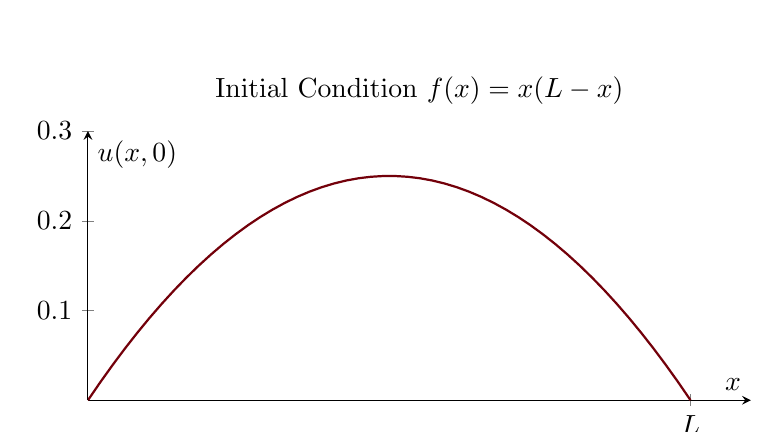
\begin{tikzpicture}[scale=1.0]
    \begin{axis}[
        axis lines=middle,
        xlabel=$x$, ylabel={$u(x,0)$},
        xmin=0, xmax=1.1,
        ymin=0, ymax=0.3,
        width=10cm, height=5cm,
        xtick={0, 1}, xticklabels={0, $L$},
        title={Initial Condition $f(x) = x(L-x)$}
    ]
    % Plotting x(1-x) as a normalized representation
    \addplot[thick, color=USC_Garnet, domain=0:1, samples=50] {x*(1-x)};
    \end{axis}
\end{tikzpicture}
\caption{Visual representation of the initial temperature distribution (parabolic profile).}
\end{figure}

\begin{stepbox}
The temporal equation is $T' + k\lambda_n T = 0$, which has the solution:
\[ T_n(t) = B_n e^{-k\lambda_n t} = B_n e^{-k(n\pi/L)^2 t} \]
Superposing these product solutions gives the general series:
\[ u(x,t) = \sum_{n=1}^{\infty} B_n \sin\left(\frac{n\pi x}{L}\right) e^{-k \left(\frac{n\pi}{L}\right)^2 t} \]
\end{stepbox}

\begin{stepbox}
We use $u(x,0) = x(L-x)$ to determine coefficients $B_n$. This is the Fourier Sine Series of $f(x) = Lx - x^2$:
\[ B_n = \frac{2}{L} \int_0^L (Lx - x^2) \sin\left(\frac{n\pi x}{L}\right) dx \]
Using integration by parts or standard tables:
\[ \int_0^L (Lx - x^2) \sin\left(\frac{n\pi x}{L}\right) dx = \frac{2L^3}{(n\pi)^3} [1 - (-1)^n] \]
Substituting this back into the expression for $B_n$:
\[ B_n = \frac{2}{L} \cdot \frac{2L^3}{(n\pi)^3} [1 - (-1)^n] = \frac{4L^2}{(n\pi)^3} [1 - (-1)^n] \]
\begin{itemize}
    \item If $n$ is even, $1 - (-1)^n = 0$, so $B_n = 0$.
    \item If $n$ is odd, $1 - (-1)^n = 2$, so $B_n = \frac{8L^2}{(n\pi)^3}$.
\end{itemize}
\end{stepbox}

\begin{resultsbox}
The solution sums only over odd integers ($n = 1, 3, 5, \dots$):

\begin{equation*}
u(x,t) = \frac{8L^2}{\pi^3} \sum_{n=1,3,5,\dots}^{\infty} \frac{1}{n^3} \sin\left(\frac{n\pi x}{L}\right) e^{-k \left(\frac{n\pi}{L}\right)^2 t}
\end{equation*}
\end{resultsbox}

\begin{codebox}
\begin{lstlisting}
% Parameters
L = 10;       % Length
k_diff = 1;   % Thermal diffusivity
x = linspace(0, L, 50);
t = linspace(0, 5, 50);
[X_mesh, T_mesh] = meshgrid(x, t);

% Initialize Solution
U = zeros(size(X_mesh));
N_terms = 20; % Number of odd terms

% Calculate Series Sum
for m = 1:N_terms
    n = 2*m - 1; % Odd indices: 1, 3, 5...
    
    Bn = (8 * L^2) / (n * pi)^3;
    lambda = (n * pi / L)^2;
    
    spatial = sin(n * pi * X_mesh / L);
    temporal = exp(-k_diff * lambda * T_mesh);
    
    U = U + Bn * spatial .* temporal;
end

% 3D Surface Plot
figure;
surf(X_mesh, T_mesh, U);
title('Heat Equation Solution u(x,t)');
xlabel('Position x');
ylabel('Time t');
zlabel('Temperature u');
colormap('jet');
shading interp;
colorbar;
view(135, 30);
\end{lstlisting}
\end{codebox}

\begin{resultsbox}
\centering
% We render the plot directly in LaTeX using PGFPlots to simulate the output
\includegraphics[width=1\linewidth]{heat_problem_a.png}

\vspace{0.5em}
\small\textit{3D visualization of the heat decay derived from the MATLAB code above.}
\end{resultsbox}

% ============================================================================
% PROBLEM 11: Exercise 12.3 Problem 10
% ============================================================================

\question{Exercise 12.3: Problem 10 (15 pts)}\label{quest:11}

\textbf{(a)} Solve the heat equation

\begin{equation*}
k\frac{\partial^2 u}{\partial x^2} = \frac{\partial u}{\partial t}, \quad 0 < x < 100, \; t > 0
\end{equation*}

subject to:
\begin{equation*}
u(0, t) = 0, \quad u(100, t) = 0, \quad u(x, 0) = \begin{cases} 0.8x & 0 \leq x \leq 50 \\ 0.8(100 - x) & 50 < x \leq 100 \end{cases}
\end{equation*}

\textbf{(b)} Use the 3D-plot application of your CAS to graph the partial sum $S_5(x, t)$ consisting of the first five nonzero terms of the solution in part (a) for $0 \leq x \leq 100$, $0 \leq t \leq 200$. Assume that $k = 1.6352$. Experiment with various three-dimensional viewing perspectives of the surface.


\begin{figure}[htbp]
\centering
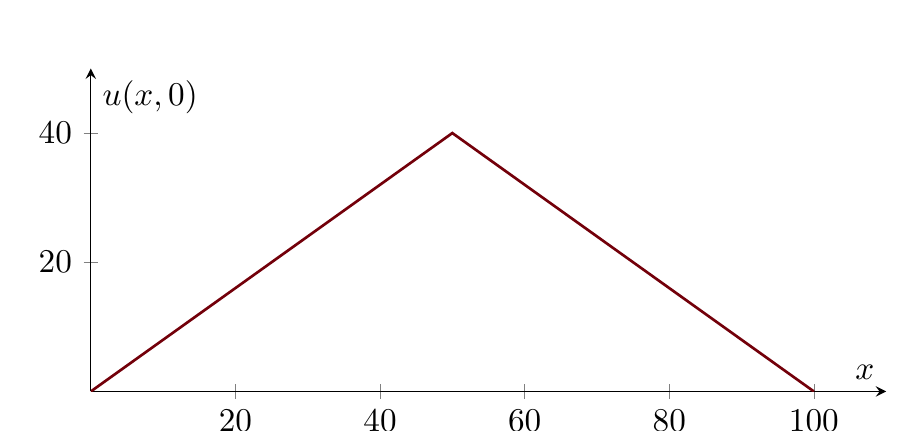
\begin{tikzpicture}[scale=1.2]
    \begin{axis}[
        axis lines=middle,
        xlabel=$x$, ylabel={$u(x,0)$},
        xmin=0, xmax=110,
        ymin=0, ymax=50,
        width=10cm, height=5cm,
        title={}
    ]
    \addplot[thick, color=USC_Garnet] coordinates {(0,0) (50,40) (100,0)};
    \end{axis}
\end{tikzpicture}
\caption{The initial temperature distribution $u(x,0)$ is a ``tent" function peaking at $u=40$ when $x=50$.}
\end{figure}

\begin{stepbox}
We assume a solution of the form $u(x,t) = X(x)T(t)$. Substituting into the heat equation $k X''T = XT'$ and separating variables:
\[ \frac{X''}{X} = \frac{T'}{kT} = -\lambda \]
This yields two ODEs:
\begin{enumerate}
    \item Spatial: $X'' + \lambda X = 0$
    \item Temporal: $T' + k\lambda T = 0$
\end{enumerate}
\end{stepbox}

\begin{stepbox}
The boundary conditions $u(0,t) = 0$ and $u(100,t) = 0$ imply $X(0) = 0$ and $X(100) = 0$.
For $X'' + \lambda X = 0$, the non-trivial solutions are sine functions:
\[ X(x) = \sin(\sqrt{\lambda} x) \]
Applying $X(100) = 0 \implies \sin(100\sqrt{\lambda}) = 0 \implies 100\sqrt{\lambda} = n\pi$.
Thus, the eigenvalues and eigenfunctions are:
\[ \lambda_n = \left(\frac{n\pi}{100}\right)^2, \quad X_n(x) = \sin\left(\frac{n\pi x}{100}\right), \quad n = 1, 2, 3, \dots \]
\end{stepbox}

\begin{stepbox}
The temporal equation is $T' + k\lambda_n T = 0$, which has the solution:
\[ T_n(t) = B_n e^{-k\lambda_n t} = B_n e^{-k (\frac{n\pi}{100})^2 t} \]
Superposing these solutions gives the general series solution:
\[ u(x,t) = \sum_{n=1}^{\infty} B_n \sin\left(\frac{n\pi x}{100}\right) e^{-k (\frac{n\pi}{100})^2 t} \]
\end{stepbox}

\begin{stepbox}
We determine $B_n$ using the initial condition $u(x,0) = f(x)$. This is the Fourier Sine Series of the tent function:
\[ B_n = \frac{2}{L} \int_0^L f(x) \sin\left(\frac{n\pi x}{L}\right) dx = \frac{2}{100} \int_0^{100} f(x) \sin\left(\frac{n\pi x}{100}\right) dx \]
Due to the symmetry of $f(x)$ about $x=50$ and the symmetry properties of sine:
\begin{itemize}
    \item If $n$ is \textbf{even}, the integrand is antisymmetric about $x=50$, so $B_n = 0$.
    \item If $n$ is \textbf{odd}, we compute the integral (using $L=100$ and peak $H=40$):
\end{itemize}
\[ B_n = \frac{2}{100} \left( \int_0^{50} 0.8x \sin\left(\frac{n\pi x}{100}\right) dx + \int_{50}^{100} 0.8(100-x) \sin\left(\frac{n\pi x}{100}\right) dx \right) \]
Evaluating this integral yields:
\[ B_n = \frac{320}{(n\pi)^2} \sin\left(\frac{n\pi}{2}\right) \quad \text{for odd } n \]
\end{stepbox}
\begin{resultsbox}
The solution considering the first five nonzero terms ($n=1, 3, 5, 7, 9$) is:

\begin{align*}
u(x,t) \approx \frac{320}{\pi^2} \bigg[ & \sin\left(\frac{\pi x}{100}\right) e^{-k(\frac{\pi}{100})^2 t} - \frac{1}{9}\sin\left(\frac{3\pi x}{100}\right) e^{-k(\frac{3\pi}{100})^2 t} \\
& + \frac{1}{25}\sin\left(\frac{5\pi x}{100}\right) e^{-k(\frac{5\pi}{100})^2 t} - \frac{1}{49}\sin\left(\frac{7\pi x}{100}\right) e^{-k(\frac{7\pi}{100})^2 t} \\
& + \frac{1}{81}\sin\left(\frac{9\pi x}{100}\right) e^{-k(\frac{9\pi}{100})^2 t} \bigg]
\end{align*}
\end{resultsbox}


\begin{codebox}
\begin{lstlisting}
% Parameters
L = 100;
k_diff = 1.6352; % Thermal diffusivity
x = linspace(0, L, 50);
t = linspace(0, 200, 50);
[X, T] = meshgrid(x, t);

% Initialize Sum
U = zeros(size(X));
N_nonzero_terms = 5; 

% Calculate Partial Sum S5
for k = 1:N_nonzero_terms
    n = 2*k - 1; % Maps k=1,2,3,4,5 to n=1,3,5,7,9
    
    % Fourier Coefficient Bn
    Bn = (320 / (n*pi)^2) * sin(n*pi/2);
    
    % Eigenvalues and Eigenfunctions
    lambda = (n*pi/L)^2;
    spatial = sin(n*pi*X/L);
    temporal = exp(-k_diff * lambda * T);
    
    U = U + Bn * spatial .* temporal;
end

% 3D Surface Plot
figure;
surf(X, T, U);
title('Partial Sum S_5(x,t) for Heat Equation');
xlabel('Position x');
ylabel('Time t');
zlabel('Temperature u');
colormap('jet');
shading interp;
colorbar;
view(135, 30); % Adjust view angle
\end{lstlisting}
\end{codebox}

\begin{resultsbox}
\centering
% We render the plot directly in LaTeX using PGFPlots to simulate the output
\includegraphics[width=1\linewidth]{heat_problem.png}

\vspace{0.5em}
\small\textit{3D surface plot of the partial sum $S_5(x,t)$ showing the decay of the initial triangular temperature profile over time.}
\end{resultsbox}

% ============================================================================
% PROBLEM 12: Exercise 12.4 Problem 11
% ============================================================================

\question{Exercise 12.4: Problem 11 (8 pts)}\label{quest:12}

The longitudinal displacement of a vibrating elastic bar satisfies the wave equation

\begin{equation*}
a^2\frac{\partial^2 u}{\partial x^2} = \frac{\partial^2 u}{\partial t^2}, \quad 0 < x < L, \; t > 0
\end{equation*}

with the boundary conditions (free-end conditions):
\begin{equation*}
\frac{\partial u}{\partial x}\bigg|_{x=0} = 0, \quad \frac{\partial u}{\partial x}\bigg|_{x=L} = 0, \quad t > 0
\end{equation*}

\begin{equation*}
u(x, 0) = x, \quad \frac{\partial u}{\partial t}\bigg|_{t=0} = 0, \quad 0 < x < L
\end{equation*}

Find the displacement $u(x,t)$.

\begin{figure}[htbp]
\centering
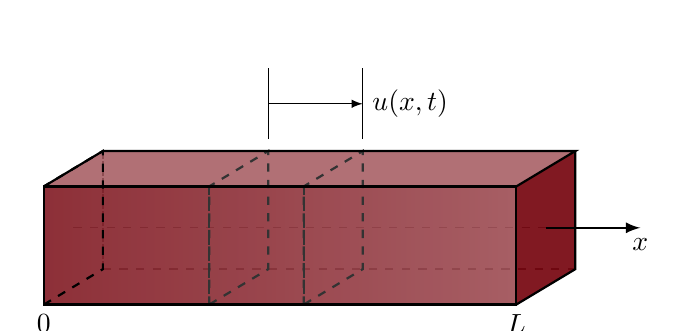
\begin{tikzpicture}[
    x={(1cm,0cm)},       % X direction
    y={(0cm,1cm)},       % Y direction
    z={(0.5cm,0.3cm)},   % Z direction (depth)
    scale=1.5,
    >=Stealth
]

    % --- Parameters ---
    \def\L{4}    % Length of the rod
    \def\H{1}    % Height
    \def\D{1}    % Depth
    \def\sStart{1.4} % Start of slice x
    \def\sEnd{2.2}   % End of slice x+dx

    % --- 1. Hidden (Back) Lines ---
    % Bottom-Back edge and Left-Back vertical edge are hidden
    \draw[dashed, thick, black!70] (0,0,\D) -- (\L,0,\D);
    \draw[dashed, thick, black!70] (0,0,\D) -- (0,\H,\D);
    \draw[dashed, thick, black!70] (0,\H,\D) -- (0,0,\D); % Left back vertical
    
    % --- 2. Centerline Axes (Longitudinal) ---
    % Central axis through the volume
    \draw[dashed, thin, black!60] (0, \H/2, \D/2) -- (\L, \H/2, \D/2);

    % --- 3. The Rod Body (Fills) ---
    
    % We apply shading. Since TikZ standard shading is 2D, we shade faces individually.
    
    % Front Face (Gradient Left to Right)
    \shade[left color=USC_Garnet!90, right color=USC_Garnet!70, opacity=0.9] 
        (0,0,0) rectangle (\L,\H,0);
        
    % Top Face (Lighter uniform yellow)
    \fill[USC_Garnet!70, opacity=0.8] 
        (0,\H,0) -- (\L,\H,0) -- (\L,\H,\D) -- (0,\H,\D) -- cycle;
        
    % Side/Right Face (Darker)
    \fill[USC_Garnet, opacity=0.9] 
        (\L,0,0) -- (\L,\H,0) -- (\L,\H,\D) -- (\L,0,\D) -- cycle;

    % --- 4. The "Slice" / Element Lines ---
    % These are the dashed cuts at x and x+dx
    
    % Slice Start
    \draw[dashed, thick, black!80] (\sStart, 0, 0) -- (\sStart, \H, 0) -- (\sStart, \H, \D) -- (\sStart, 0, \D) -- cycle;
    \draw[dashed, thick, black!80] (\sStart, \H, 0) -- (\sStart, 0, 0); % Front face vertical
    
    % Slice End
    \draw[dashed, thick, black!80] (\sEnd, 0, 0) -- (\sEnd, \H, 0) -- (\sEnd, \H, \D) -- (\sEnd, 0, \D) -- cycle;
    \draw[dashed, thick, black!80] (\sEnd, \H, 0) -- (\sEnd, 0, 0); % Front face vertical

    % --- 5. Visible Edges (Outlines) ---
    \draw[thick] (0,0,0) -- (\L,0,0) -- (\L,\H,0) -- (0,\H,0) -- cycle; % Front face border
    \draw[thick] (0,\H,0) -- (0,\H,\D) -- (\L,\H,\D) -- (\L,\H,0);     % Top edges
    \draw[thick] (\L,0,0) -- (\L,0,\D) -- (\L,\H,\D);                   % Right edges
    \draw[thick, dashed] (0,0,0) -- (0,0,\D) -- (0,\H,\D) -- (0,\H,0);  % Left edges (partially dashed in standard view, but strict outline here)

    % --- 6. Annotations ---

    % Coordinates Labels
    \node[below] at (0,0,0) {$0$};
    \node[below] at (\L,0,0) {$L$};

    % X-Axis Arrow
    \draw[-latex, thick] (\L, \H/2, \D/2) -- ++(0.8, 0, 0) node[below] {$x$};

    % Dimension lines for u(x,t)
    % Extension lines going up
    \draw[thin, black] (\sStart, \H+0.1, \D) -- ++(0, 0.6, 0);
    \draw[thin, black] (\sEnd, \H+0.1, \D) -- ++(0, 0.6, 0);

    % Arrow and Label
    \draw[-latex, thin] (\sStart, \H+0.4, \D) -- node[right, xshift=6mm] {$u(x,t)$} ++(0.8, 0, 0);
    
    % Note: In the original image, the arrow starts at the left slice boundary 
    % and points right, indicating displacement direction.

\end{tikzpicture}
    \caption{3D view of the rod with a differential slice between $x$ and $x + \Delta x$.}
    \label{fig:rod-slice}
\end{figure}
\begin{stepbox}
We assume a solution of the form $u(x,t) = X(x)T(t)$. Substituting this into the wave equation $a^2 u_{xx} = u_{tt}$ gives:
\[ a^2 X''(x)T(t) = X(x)T''(t) \]
Dividing by $a^2 X(x)T(t)$, we separate the variables to equal a constant $-\lambda$:
\[ \frac{X''(x)}{X(x)} = \frac{1}{a^2}\frac{T''(t)}{T(t)} = -\lambda \]
This yields two ordinary differential equations:
\begin{enumerate}
    \item Spatial: $X''(x) + \lambda X(x) = 0$
    \item Temporal: $T''(t) + a^2\lambda T(t) = 0$
\end{enumerate}
\end{stepbox}

\begin{stepbox}
Boundary conditions: $u_x(0,t) = 0 \implies X'(0)=0$ and $u_x(L,t)=0 \implies X'(L)=0$.

\begin{itemize}
    \item \textbf{Case $\lambda = 0$:} $X(x) = c_1 x + c_2$. $X'(x) = c_1$.
    $X'(0)=0 \implies c_1=0$. $X'(L)=0$ is satisfied.
    Eigenfunction: $X_0(x) = 1$ (constant).
    
    \item \textbf{Case $\lambda > 0$:} Let $\lambda = \beta^2$. $X(x) = A \cos(\beta x) + B \sin(\beta x)$.
    $X'(x) = -A\beta \sin(\beta x) + B\beta \cos(\beta x)$.
    $X'(0) = B\beta = 0 \implies B=0$.
    $X'(L) = -A\beta \sin(\beta L) = 0 \implies \beta L = n\pi$.
    Eigenvalues: $\lambda_n = (\frac{n\pi}{L})^2$. Eigenfunctions: $X_n(x) = \cos(\frac{n\pi x}{L})$.
\end{itemize}
\end{stepbox}

\begin{stepbox}
\begin{itemize}
    \item For $\lambda_0=0$: $T''(t)=0 \implies T_0(t) = \frac{A_0}{2} + \frac{B_0}{2}t$.
    \item For $\lambda_n > 0$: $T_n(t) = A_n \cos(\frac{n\pi a t}{L}) + B_n \sin(\frac{n\pi a t}{L})$.
\end{itemize}

Applying initial velocity $\frac{\partial u}{\partial t}\big|_{t=0} = 0$:
\[ \frac{\partial u}{\partial t}(x,0) = \frac{B_0}{2} + \sum \frac{n\pi a}{L} B_n \cos\left(\frac{n\pi x}{L}\right) = 0 \]
By orthogonality, $B_0 = 0$ and all $B_n = 0$.
The series reduces to:
\[ u(x,t) = \frac{A_0}{2} + \sum_{n=1}^{\infty} A_n \cos\left(\frac{n\pi a t}{L}\right) \cos\left(\frac{n\pi x}{L}\right) \]
\end{stepbox}

\begin{stepbox}
We use $u(x,0) = x$ to find $A_n$ via Fourier Cosine Series.

\[ A_0 = \frac{2}{L} \int_0^L x \, dx = \frac{2}{L} \left[\frac{x^2}{2}\right]_0^L = L \]
\[ A_n = \frac{2}{L} \int_0^L x \cos\left(\frac{n\pi x}{L}\right) dx \]
Using integration by parts:
\[ A_n = \frac{2}{L} \left[ \frac{Lx}{n\pi}\sin\left(\frac{n\pi x}{L}\right) + \frac{L^2}{(n\pi)^2}\cos\left(\frac{n\pi x}{L}\right) \right]_0^L \]
\[ A_n = \frac{2L}{(n\pi)^2} [(-1)^n - 1] \]
If $n$ is even, $A_n = 0$. If $n$ is odd, $A_n = -\frac{4L}{(n\pi)^2}$.
\end{stepbox}


\begin{resultsbox}
The final displacement solution summing over odd integers $n$:
\begin{equation*}
u(x,t) = \frac{L}{2} - \frac{4L}{\pi^2} \sum_{n=1, 3, 5, \dots}^{\infty} \frac{1}{n^2} \cos\left(\frac{n\pi a t}{L}\right) \cos\left(\frac{n\pi x}{L}\right)
\end{equation*}
\end{resultsbox}


\begin{codebox}
\begin{lstlisting}
import numpy as np
import matplotlib.pyplot as plt

# Parameters
L = 1.0
a = 1.0
x = np.linspace(0, L, 100)
t_values = [0, 0.5] 
N_terms = 20 

plt.figure()
# Calculate Series Sum
for t in t_values:
    u = np.full_like(x, L/2) # Start with constant A0/2
    for k in range(1, N_terms + 1):
        n = 2*k - 1 # Odd terms only
        An = -4*L / (np.pi**2 * n**2)
        spatial = np.cos(n * np.pi * x / L)
        temporal = np.cos(n * np.pi * a * t / L)
        u += An * spatial * temporal
    plt.plot(x, u, label=f't={t}')

plt.title('Displacement u(x,t)')
plt.legend()
plt.show()
\end{lstlisting}
\end{codebox}

\begin{resultsbox}
\centering
% We render the plot directly in LaTeX using PGFPlots to simulate the output
\includegraphics[width=1\linewidth]{problem_elastic.png}

\vspace{0.5em}
\small\textit{At $t=0$, the series converges to the initial linear displacement. As time evolves, the bar oscillates around the average displacement $L/2$}
\end{resultsbox}


% ============================================================================
% PROBLEM 13: Exercise 12.5 Problem 16
% ============================================================================

\question{Exercise 12.5: Problem 16 (12 pts)}\label{quest:13}

Use the superposition principle to solve Laplace's equation

\begin{equation*}
\frac{\partial^2 u}{\partial x^2} + \frac{\partial^2 u}{\partial y^2} = 0, \quad 0 < x < 2, \; 0 < y < 2
\end{equation*}

for a square plate subject to the given boundary conditions:

\begin{equation*}
u(0, y) = 0, \quad u(2, y) = y(2 - y)
\end{equation*}

\begin{equation*}
u(x, 0) = 0, \quad u(x, 2) = \begin{cases} x & 0 < x < 1 \\ 2 - x & 1 \leq x < 2 \end{cases}
\end{equation*}

\begin{stepbox}
Since Laplace's equation is linear, we can express the solution $u(x,y)$ as the sum of two simpler solutions, $u_1(x,y)$ and $u_2(x,y)$, such that:
\[ u(x,y) = u_1(x,y) + u_2(x,y) \]

\textbf{Problem 1 ($u_1$): Non-homogeneous on Top Boundary ($y=2$)}
\begin{itemize}
    \item $u_1(0,y) = 0$, $u_1(2,y) = 0$
    \item $u_1(x,0) = 0$
    \item $u_1(x,2) = f(x)$ (The tent function)
\end{itemize}

\textbf{Problem 2 ($u_2$): Non-homogeneous on Right Boundary ($x=2$)}
\begin{itemize}
    \item $u_2(0,y) = 0$
    \item $u_2(x,0) = 0$, $u_2(x,2) = 0$
    \item $u_2(2,y) = g(y) = y(2-y)$
\end{itemize}
\end{stepbox}

\begin{stepbox}
Using separation of variables $u_1(x,y) = X(x)Y(y)$, we obtain $X'' + \lambda X = 0$ and $Y'' - \lambda Y = 0$.
Due to zero boundary conditions at $x=0$ and $x=2$, we find eigenvalues $\lambda_n = (\frac{n\pi}{2})^2$ and eigenfunctions $X_n(x) = \sin(\frac{n\pi x}{2})$.
The solution takes the form:
\[ u_1(x,y) = \sum_{n=1}^{\infty} A_n \sin\left(\frac{n\pi x}{2}\right) \sinh\left(\frac{n\pi y}{2}\right) \]

Applying $u_1(x,2) = f(x)$, we find coefficients $A_n$:
\[ A_n \sinh(n\pi) = \frac{2}{2} \int_0^2 f(x) \sin\left(\frac{n\pi x}{2}\right) dx \]
For the symmetric tent function $f(x)$, the Fourier sine coefficients are non-zero only for odd $n$:
\[ A_n \sinh(n\pi) = \frac{8}{(n\pi)^2} \sin\left(\frac{n\pi}{2}\right) \implies A_n = \frac{8 \sin(n\pi/2)}{(n\pi)^2 \sinh(n\pi)} \]
\end{stepbox}

\begin{stepbox}
Similarly, for $u_2$, the homogeneous conditions are on $y=0, y=2$ and $x=0$. The form is:
\[ u_2(x,y) = \sum_{n=1}^{\infty} B_n \sinh\left(\frac{n\pi x}{2}\right) \sin\left(\frac{n\pi y}{2}\right) \]

Applying $u_2(2,y) = y(2-y)$, we find coefficients $B_n$:
\[ B_n \sinh(n\pi) = \frac{2}{2} \int_0^2 (2y - y^2) \sin\left(\frac{n\pi y}{2}\right) dy \]
Evaluating this integral yields (for odd $n$):
\[ B_n \sinh(n\pi) = \frac{32}{(n\pi)^3} \implies B_n = \frac{32}{(n\pi)^3 \sinh(n\pi)} \]
\end{stepbox}

\begin{resultsbox}
The total solution is the sum of the two series (summing over odd $n$):
\begin{align*}
u(x,y) &= \sum_{n=1,3,5\dots}^{\infty} \left[ \frac{8 \sin(\frac{n\pi}{2})}{(n\pi)^2 \sinh(n\pi)} \sin\left(\frac{n\pi x}{2}\right) \sinh\left(\frac{n\pi y}{2}\right) \right] \\
       &+ \sum_{n=1,3,5\dots}^{\infty} \left[ \frac{32}{(n\pi)^3 \sinh(n\pi)} \sinh\left(\frac{n\pi x}{2}\right) \sin\left(\frac{n\pi y}{2}\right) \right]
\end{align*}
\end{resultsbox}

\newpage

\begin{codebox}
\begin{lstlisting}
% Parameters
L = 2;
N_terms = 50; % Number of series terms
[X, Y] = meshgrid(linspace(0, 2, 50), linspace(0, 2, 50));
U = zeros(size(X));

% Calculate Series Sum
for n = 1:2:N_terms  % Odd n only
    lam = n * pi / 2;
    sinh_term = sinh(n * pi);
    
    % u1 Coefficients (Tent function on Top)
    An = (8 * sin(n*pi/2)) / ((n*pi)^2 * sinh_term);
    U1 = An * sin(lam * X) .* sinh(lam * Y);
    
    % u2 Coefficients (Parabola on Right)
    Bn = 32 / ((n*pi)^3 * sinh_term);
    U2 = Bn * sinh(lam * X) .* sin(lam * Y);
    
    U = U + U1 + U2;
end

% Visualization
figure;
surf(X, Y, U);
title('Steady State Temperature Distribution u(x,y)');
xlabel('x'); ylabel('y'); zlabel('u');
colormap('jet'); shading interp;
\end{lstlisting}
\end{codebox}

\begin{resultsbox}
\centering
% We render the plot directly in LaTeX using PGFPlots to simulate the output
\includegraphics[width=1\linewidth]{problem_laplace.png}

\vspace{0.5em}
\small\textit{3D surface plot generated from the first two odd harmonics of the derived series.}
\end{resultsbox}

% ============================================================================
% END OF DOCUMENT
% ============================================================================

\end{document}
